\documentclass[11pt]{article}

\title{Homework 5 -- ECE 594E}

\author{Steven Munn}

\usepackage{datetime}
\usepackage{amsmath}
\usepackage{tikz}
\usetikzlibrary{arrows,automata,positioning}
\usepackage{graphicx}
\usepackage{hyperref}


\newcommand{\abs}[1]{\mathopen|#1\mathclose|}
\newcommand{\mb}[1]{\mathbf{#1}}
\newdate{date}{25}{11}{2014}
\date{Due \displaydate{date}}

\begin{document}

\maketitle

\section{Particle Filter for non-linear system}
\subsection{}

We plot two sample trajectories in figures \ref{st1} and \ref{st2}.

\begin{figure}[h]
  
  \centering
    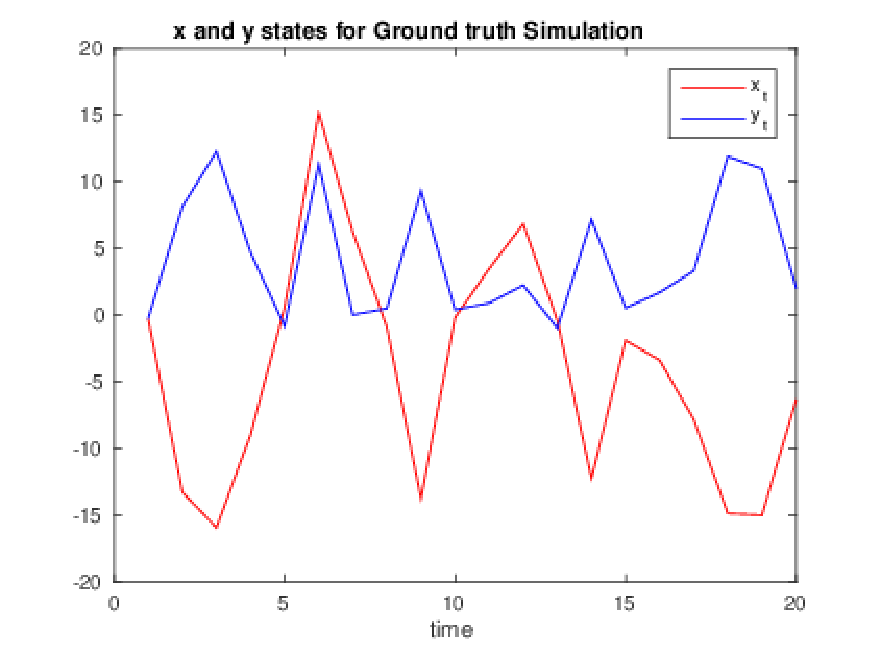
\includegraphics[width=80mm]{../figs/001_11_sampletraj1.pdf}
    \caption{First sample trajectory}
    \label{st1}
\end{figure}

\begin{figure}[h]
  
  \centering
    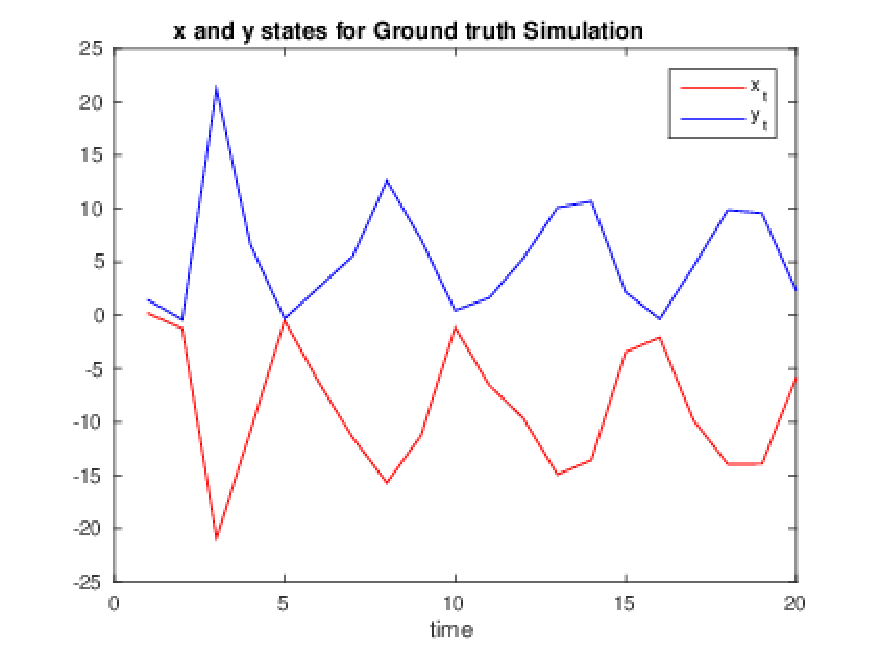
\includegraphics[width=80mm]{../figs/002_11_sampletraj2.pdf}
    \caption{Second sample trajectory}
    \label{st2}
\end{figure}

\subsection{}

The full implementation code can be found at \url{https://github.com/stevenjlm/ML-code/tree/master/bootstrap}

\subsection{}

For $N=100$ particles, using measurements $y_t$, $t=1$ to $t=T=100$ we plot the conditional mean and the actual state in figure \ref{bs}. The mean square error between estimate and actual state is in figure \ref{mse}.

In figures \ref{t10}, \ref{t50}, and \ref{t100} we plot $p(x_{t}|y_{1:T})$ at times 10, 50, and 100. Only the plot at time 100 is bimodal, this mostly coincidence though. You can see in figure \ref{t50} that the peak is very close to zero. The distribution is a mixture of two Gaussians, it's just that their means are too close to produce distinguishable peaks. And, for figure \ref{t10} the value is so extremely low that the state must have been in a downward slope already and the step function didn't produce particles at the other mode peak.

\begin{figure}[h]
  
  \centering
    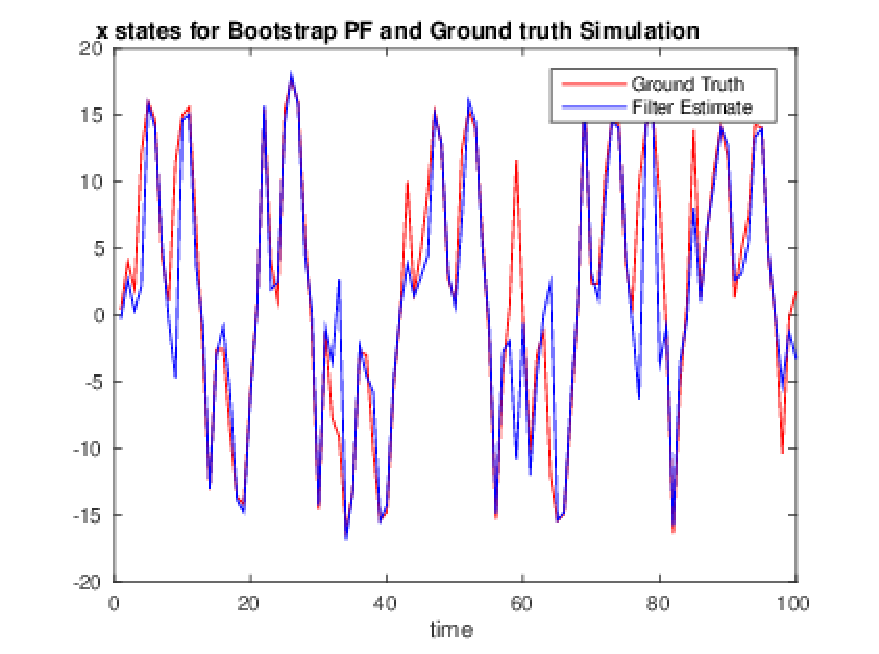
\includegraphics[width=80mm]{../figs/003_13_gt-and-bt.pdf}
    \caption{Particle Filter estimate and actual state}
    \label{bs}
\end{figure}

\begin{figure}[h]
  
  \centering
    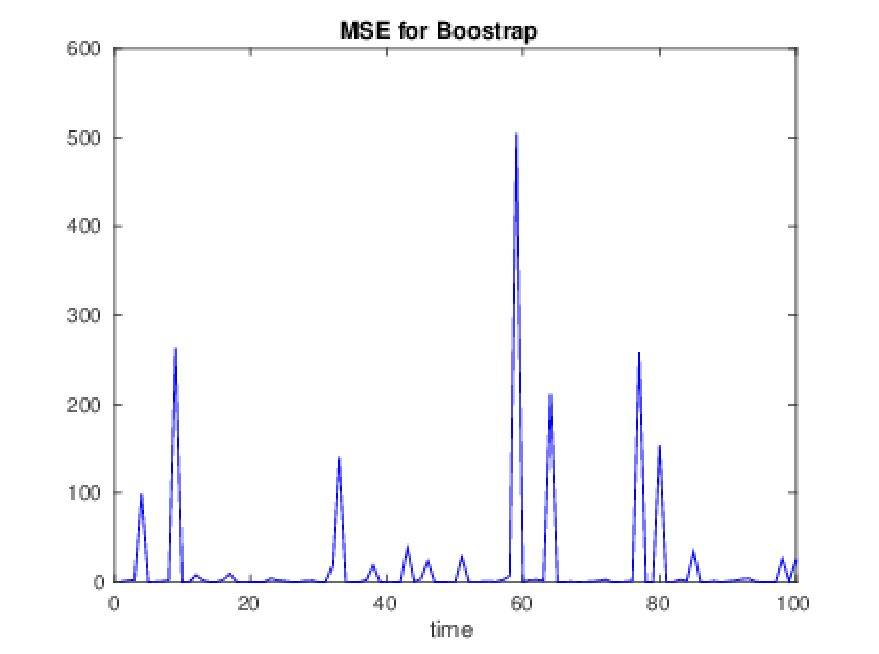
\includegraphics[width=80mm]{../figs/004_13_mse.pdf}
    \caption{Mean square error of estimate}
    \label{mse}
\end{figure}

\begin{figure}[h]
  
  \centering
    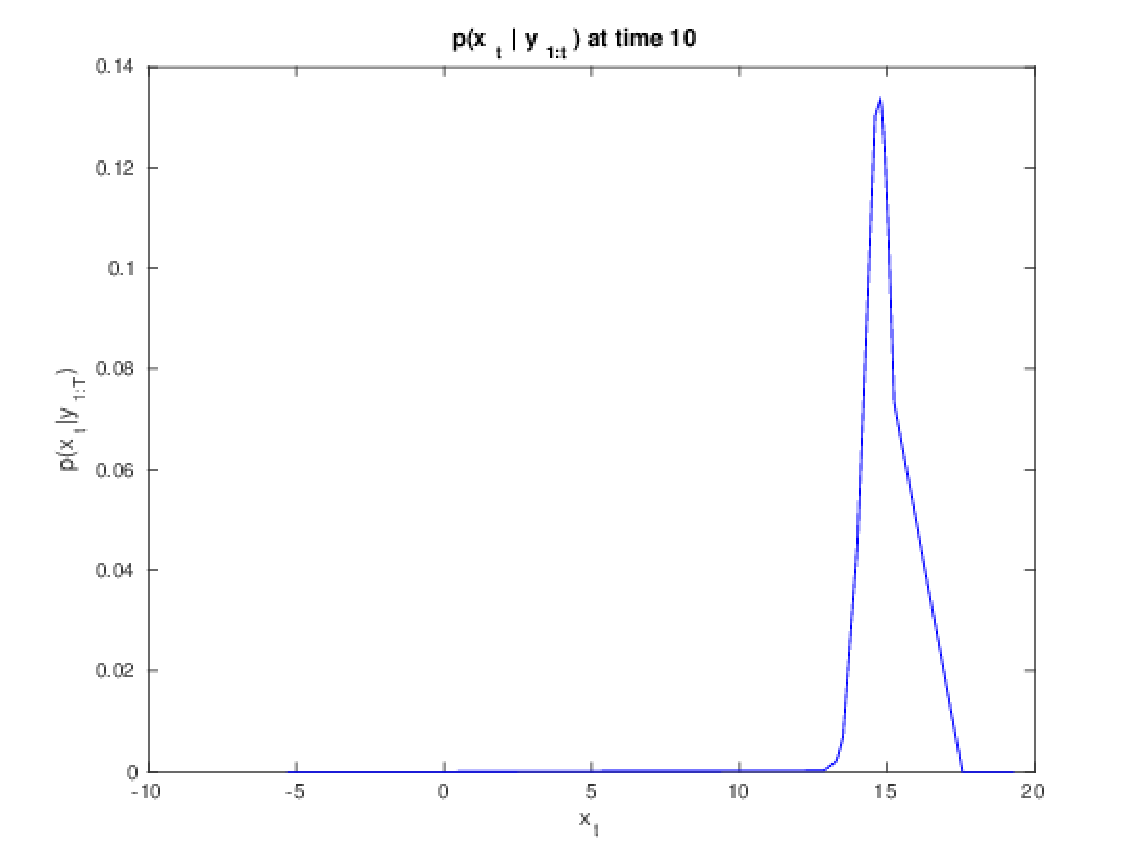
\includegraphics[width=80mm]{../figs/005_13_t10.pdf}
    \caption{Filtering density at $t=10$}
    \label{t10}
\end{figure}

\begin{figure}[h]
  
  \centering
    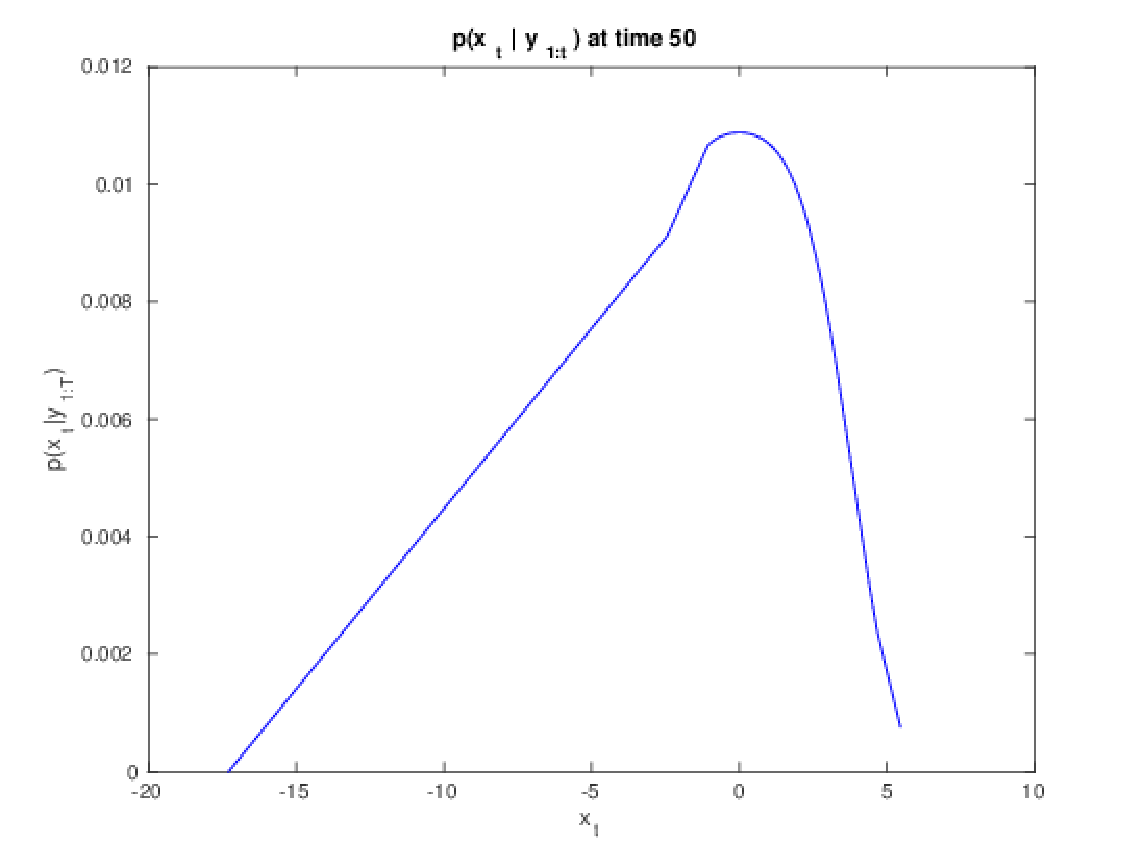
\includegraphics[width=80mm]{../figs/006_13_t50.pdf}
    \caption{Filtering density at $t=50$}
    \label{t50}
\end{figure}

\begin{figure}[h]
  
  \centering
    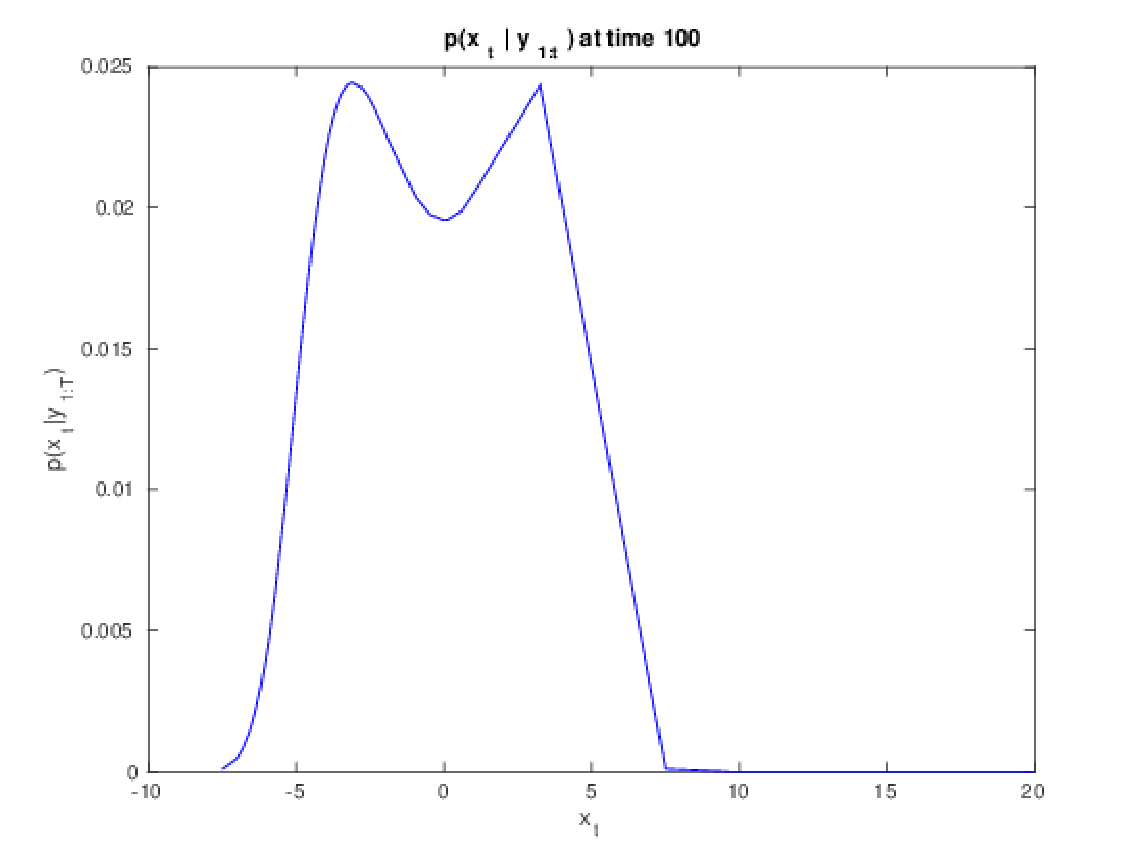
\includegraphics[width=80mm]{../figs/007_13_t100.pdf}
    \caption{Filtering density at $t=100$}
    \label{t100}
\end{figure}

\subsection{}

For $N=10$ we have the same plots as above in figures \ref{n10gtbt}, \ref{n10gtbt}, \ref{n101}, \ref{n102}, \ref{n103}, and \ref{n104}.

\begin{figure}[h]
  
  \centering
    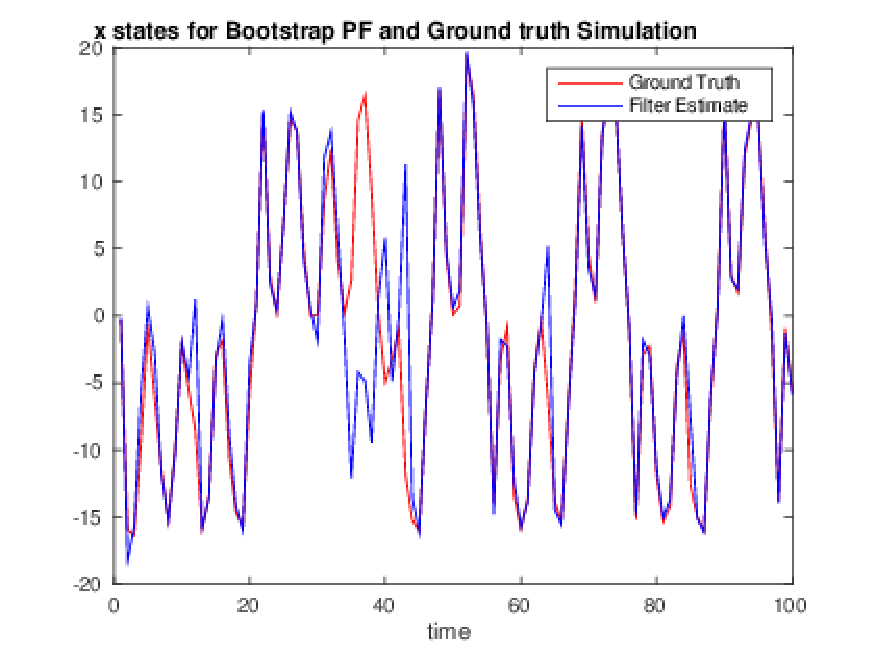
\includegraphics[width=80mm]{../figs/008_15_gt-and-bt.pdf}
    \caption{Particle Filter estimate and actual state}
    \label{n10gtbt}
\end{figure}

\begin{figure}[h]
  
  \centering
    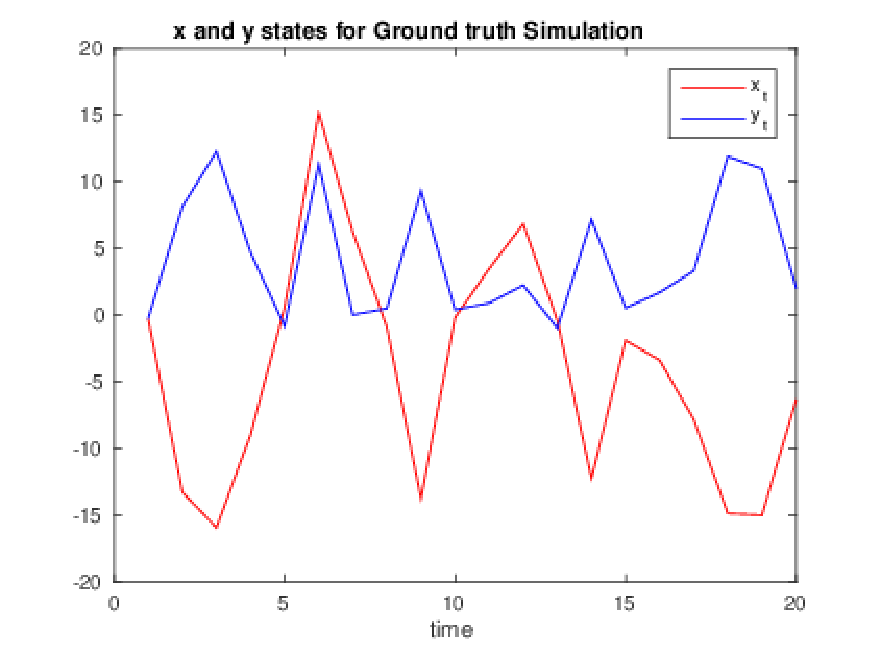
\includegraphics[width=80mm]{../figs/009_13_mse.pdf}
    \caption{Mean square error of estimate}
    \label{n101}
\end{figure}

\begin{figure}[h]
  
  \centering
    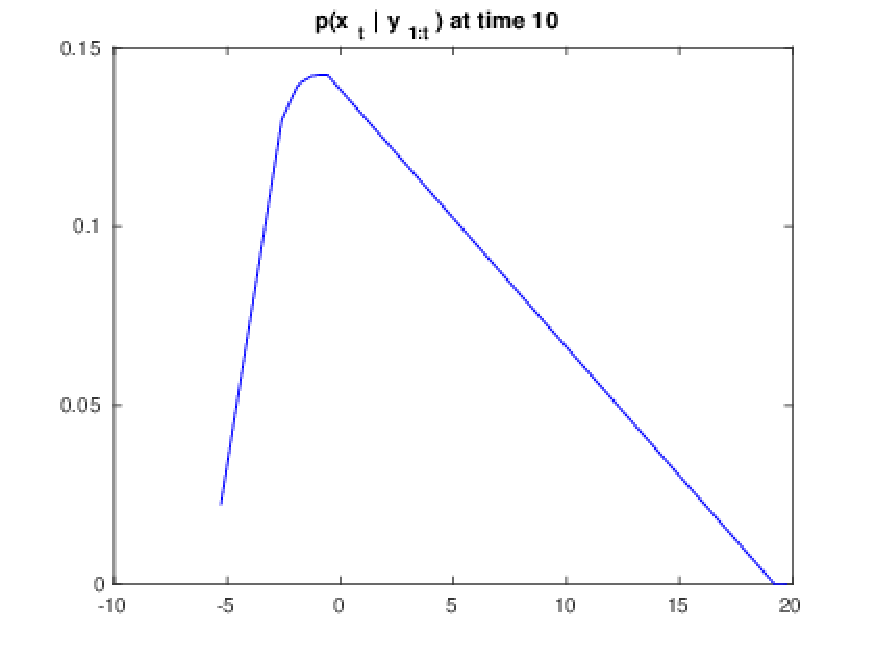
\includegraphics[width=80mm]{../figs/010_15_t10N10.pdf}
    \caption{Filtering density at $t=10$}
    \label{n102}
\end{figure}

\begin{figure}[h]
  
  \centering
    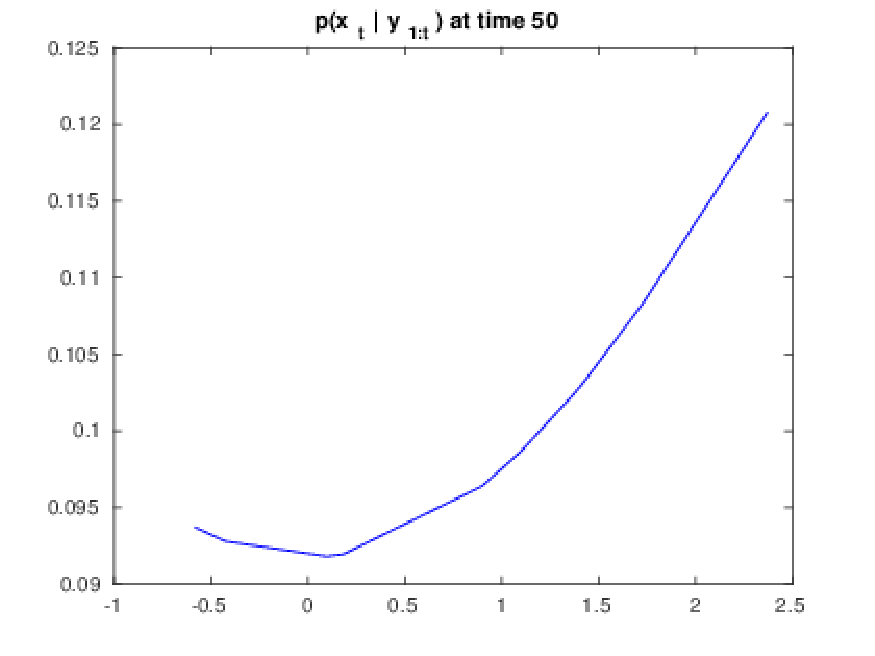
\includegraphics[width=80mm]{../figs/011_15_t50N10.pdf}
    \caption{Filtering density at $t=50$}
    \label{n103}
\end{figure}

\begin{figure}[h]
  
  \centering
    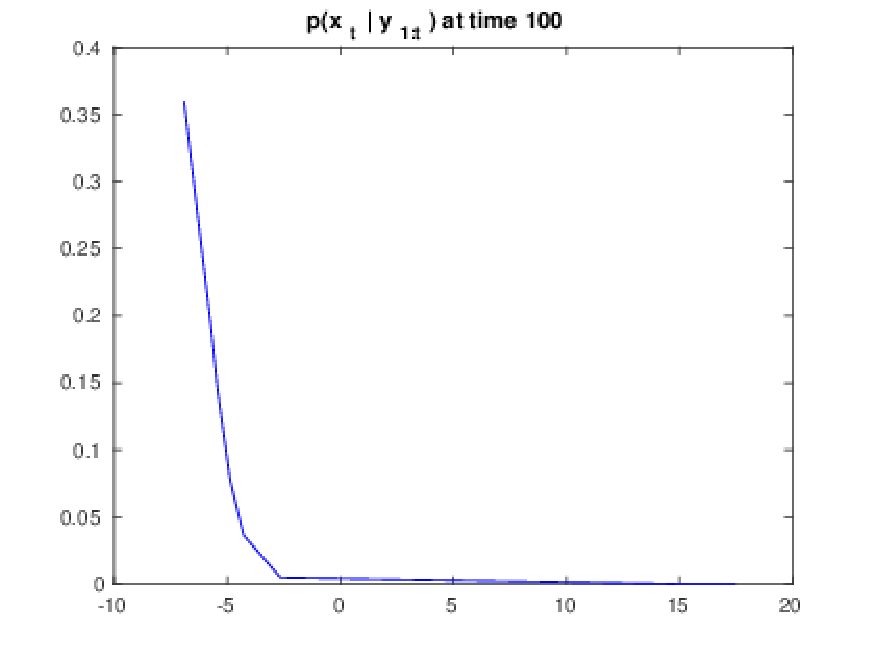
\includegraphics[width=80mm]{../figs/012_15_t100N10.pdf}
    \caption{Filtering density at $t=100$}
    \label{n104}
\end{figure}


For $N=1000$ we have the same plots as above in figures \ref{n1000gtbt}, \ref{n1000gtbt}, \ref{n10001}, \ref{n10002}, \ref{n10003}, and \ref{n10004}.

\begin{figure}[h]
  
  \centering
    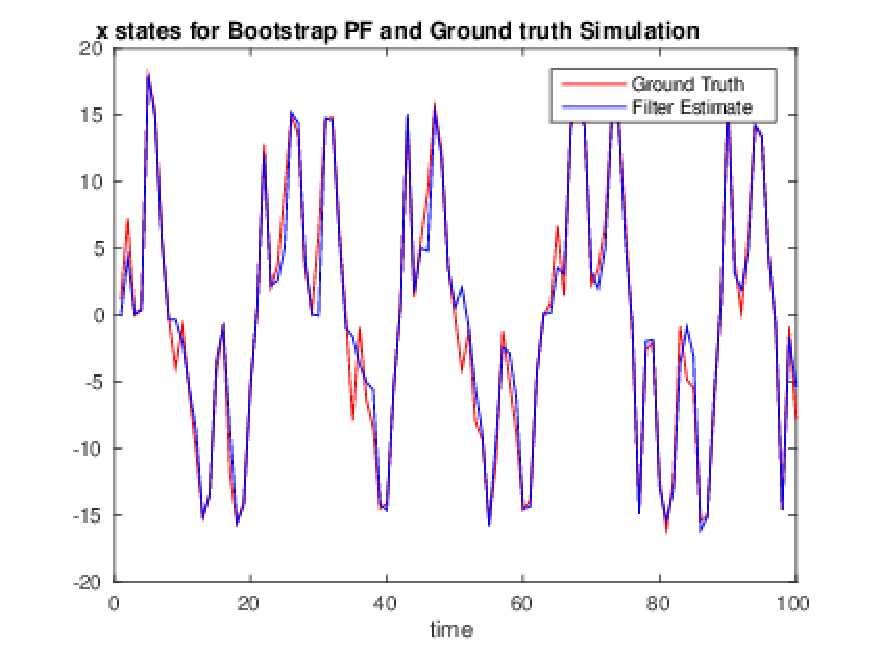
\includegraphics[width=80mm]{../figs/013_15_gt-and-bt.pdf}
    \caption{Particle Filter estimate and actual state}
    \label{n1000gtbt}
\end{figure}

\begin{figure}[h]
  
  \centering
    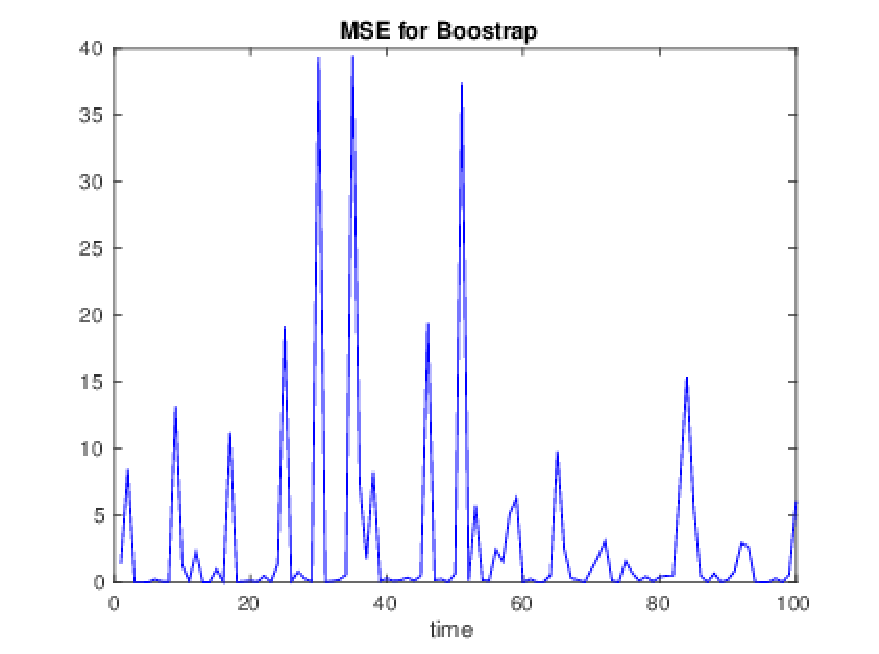
\includegraphics[width=80mm]{../figs/014_15_mseN1000.pdf}
    \caption{Mean square error of estimate}
    \label{n10001}
\end{figure}

\begin{figure}[h]
  
  \centering
    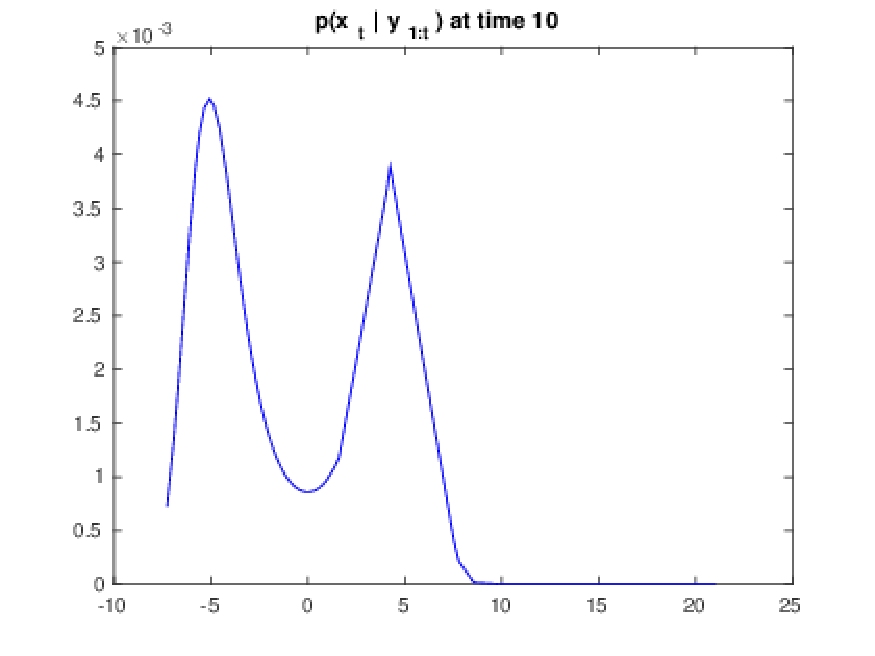
\includegraphics[width=80mm]{../figs/015_15_t10N1000.pdf}
    \caption{Filtering density at $t=10$}
    \label{n10002}
\end{figure}

\begin{figure}[h]
  
  \centering
    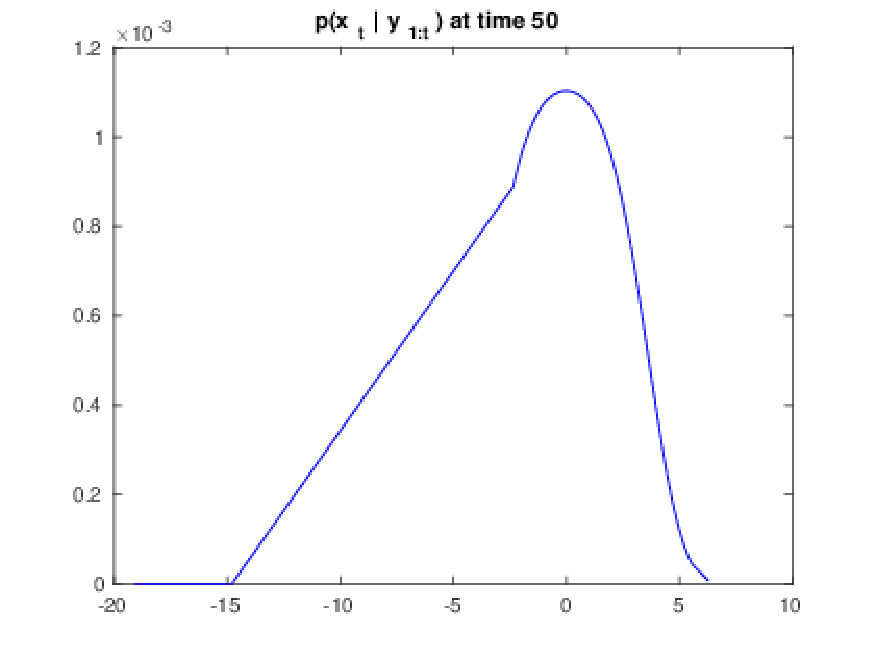
\includegraphics[width=80mm]{../figs/016_15_t50N1000.pdf}
    \caption{Filtering density at $t=50$}
    \label{n10003}
\end{figure}

\begin{figure}[h]
  
  \centering
    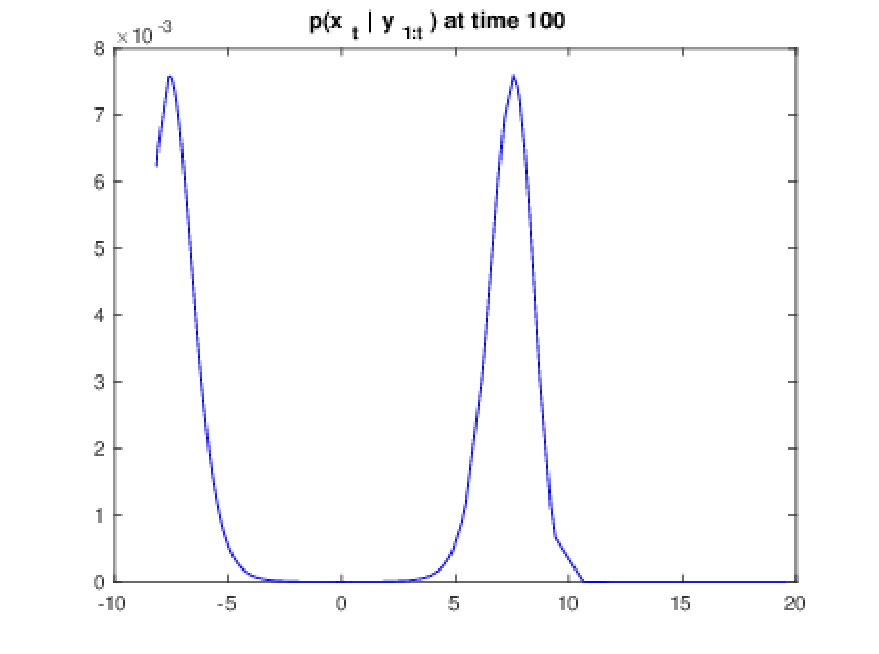
\includegraphics[width=80mm]{../figs/017_15_t100N1000.pdf}
    \caption{Filtering density at $t=100$}
    \label{n10004}
\end{figure}

\subsection{}

Backward filter is implemented in the same runme.m file as the bootstrap filter. Figure \ref{bk} shows the actual state and some sample backward trajectories.

\begin{figure}[h]
  
  \centering
    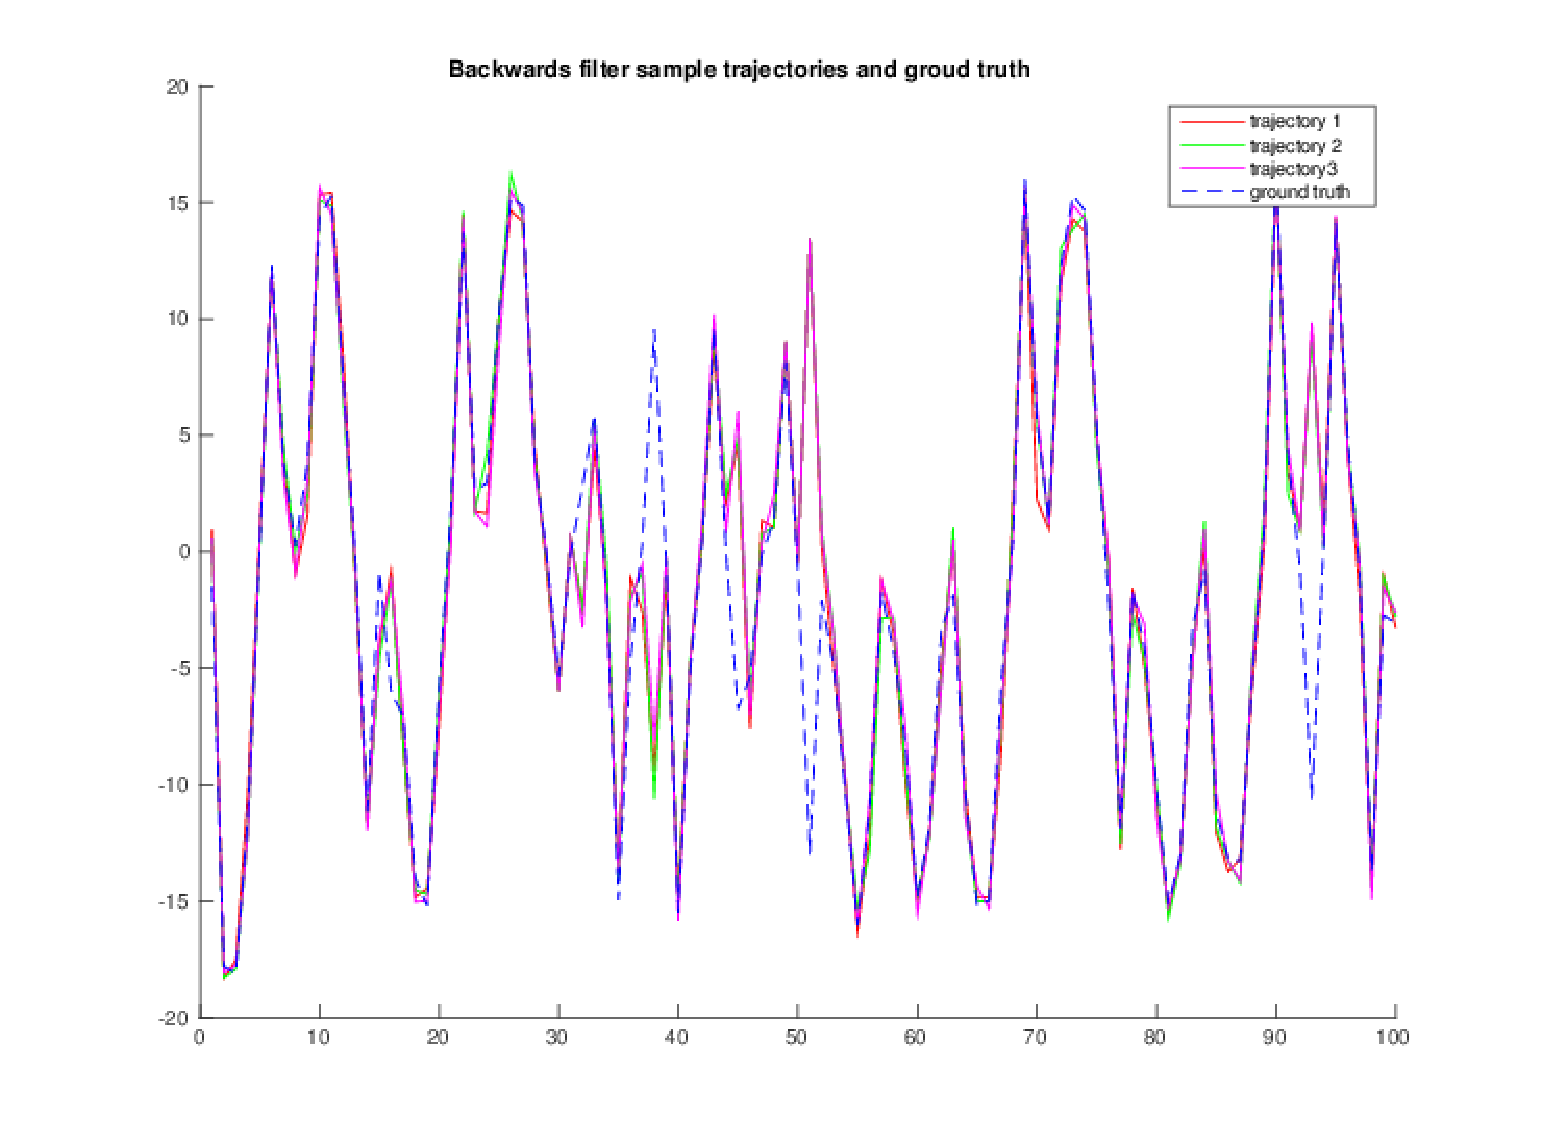
\includegraphics[width=80mm]{../figs/018_16bksam.pdf}
    \caption{Backwards Filtering sample trajectories and actual trajectory.}
    \label{bk}
\end{figure}

\subsection{}

The mean square error over the average of forward filtered particles is 0.3012 and the backward filter gets 0.2561.

\subsection{}

With $N=10$ backward particles, the MSE is hardly any better after backward filtering. With $N=100$ particles however, the MSE is significantly better since it goes down nearly one third.

\section{Kalman Filtering}

\subsection{}

The full implementation code can be found at \url{https://github.com/stevenjlm/ML-code/tree/master/kalman}



\end{document}